\section{RQ1: The Cost of the Implementation}
\label{sec:rq1}

\paragraph{Placement.} Fig.~\ref{fig:placer} shows the time of one placement of a complete B*-Tree with randomly sized modules. The original contour, a sorted set of all placed modules, is superlinear: 256 times more modules take 3200 times longer, roughly $n^{1.46}$. The original edition measured the same behaviour (Table~5.1 of the original edition shows growth by a factor of 1.9--3.1 per doubling) but concluded that it was close to linear. The array contour is linear, as the analysis of Section~\ref{sec:placement} predicts. Together with the array B*-Tree it is 7 times faster than the original placement for 100 modules and 99 times faster for 25\,600 modules.

\begin{figure}
\centering
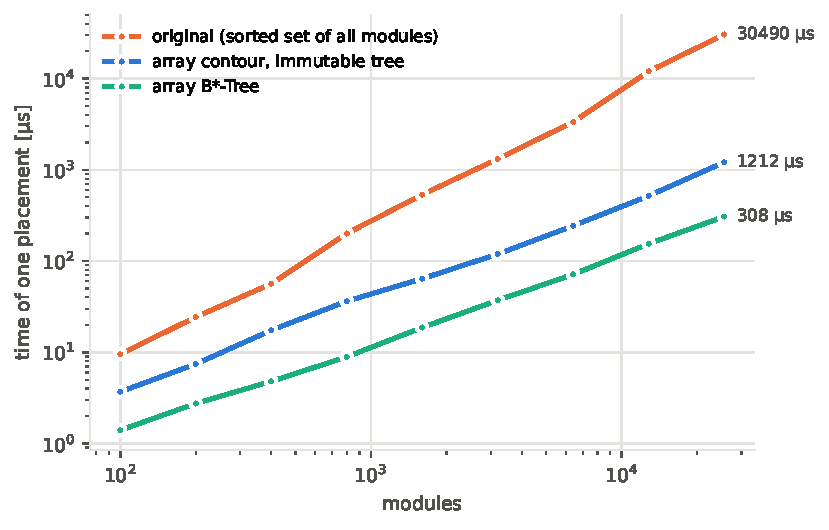
\includegraphics[width=.8\textwidth]{new/placer}
\caption{Time of one placement of a complete B*-Tree with random module sizes: the original contour, the array contour with the immutable tree, and the array B*-Tree (median of 9 batches after a warm-up; logarithmic axes)}
\label{fig:placer}
\end{figure}

\paragraph{Evaluation speed.} Table~\ref{tab:speed} shows how many floorplans per second the algorithms evaluate on the benchmarks. The optimisations of the immutable implementation, which do not change the results, make POEMS 4--8 times faster; the speed-up grows with the number of modules because the original placement is superlinear. The corrections do not change the speed. The array evaluation adds another factor of 1.7 to 3.7, so that POEMS evaluates 7.5 to 29 times more floorplans per second than the original implementation. LA-POEMS, which does not create any objects per step and stops the placement of rejected candidates early, makes 9 to 37 times more evaluations per second than the original implementation, but many of them are only partial placements.

\begin{table}
\centering
\small
\begin{tabular}{@{}lrrrrr@{}}
\toprule
Benchmark & Original & Optimised & Corrected & Array & LA-POEMS \\
\midrule
xerox & 184 & 796 \ (4.3$\times$) & 791 \ (4.3$\times$) & 1379 \ (7.5$\times$) & 1642 \ (8.9$\times$) \\
hp & 165 & 791 \ (4.8$\times$) & 745 \ (4.5$\times$) & 1319 \ (8.0$\times$) & 1680 \ (10.2$\times$) \\
ami33 & 54 & 383 \ (7.1$\times$) & 382 \ (7.0$\times$) & 848 \ (15.7$\times$) & 1117 \ (20.6$\times$) \\
ami49 & 54 & 297 \ (5.5$\times$) & 263 \ (4.9$\times$) & 698 \ (13.0$\times$) & 869 \ (16.2$\times$) \\
n100 & 24 & 156 \ (6.5$\times$) & 147 \ (6.1$\times$) & 447 \ (18.6$\times$) & 546 \ (22.7$\times$) \\
n200 & 10 & 79 \ (7.8$\times$) & 73 \ (7.3$\times$) & 253 \ (25.1$\times$) & 323 \ (32.1$\times$) \\
n300 & 6 & 48 \ (7.8$\times$) & 49 \ (8.0$\times$) & 179 \ (29.1$\times$) & 227 \ (36.8$\times$) \\
\bottomrule
\end{tabular}
\caption{Evaluations per second (thousands) of the original implementation of POEMS, the optimised implementation, the corrected one, the corrected one with the array evaluation, and LA-POEMS, whose evaluations stop early when the candidate is rejected (mean of the 30\,s runs; speed-up relative to the original implementation in parentheses)}
\label{tab:speed}
\end{table}


\paragraph{Quality.} Table~\ref{tab:rq1quality} compares the original implementation with the optimised one. Both run the same algorithm with the same seeds, so the only difference is the number of evaluations made in the 30 seconds. The faster implementation finds significantly better floorplans on all five benchmarks with more than 30 modules; for example, the mean dead space on n300 drops from 13.1\,\% to 9.0\,\%.

\begin{table}
\centering
\small
\begin{tabular}{@{}lcc@{}}
\toprule
Benchmark & Original & Optimised \\
\midrule
apte & $0.78_{\pm 0.00}\ (0.78)$ & $0.78_{\pm 0.00}\ (0.78)$ \\
xerox & $3.41_{\pm 0.58}\ (2.50)$ & $3.07_{\pm 0.41}\ (2.34)$ \\
hp & $5.23_{\pm 1.05}\ (3.88)$ & $4.43_{\pm 1.08}\ (2.28)$ \\
ami33 & $4.19_{\pm 0.73}\ (2.91)$ & $\mathbf{2.58_{\pm 0.46}\ (1.73)}$ \\
ami49 & $4.90_{\pm 0.71}\ (3.70)$ & $\mathbf{3.37_{\pm 0.64}\ (2.31)}$ \\
n100 & $6.88_{\pm 1.42}\ (5.61)$ & $\mathbf{4.15_{\pm 0.60}\ (3.49)}$ \\
n200 & $11.97_{\pm 1.15}\ (10.30)$ & $\mathbf{7.30_{\pm 0.47}\ (6.67)}$ \\
n300 & $13.09_{\pm 1.03}\ (12.02)$ & $\mathbf{9.00_{\pm 0.51}\ (7.99)}$ \\
\bottomrule
\end{tabular}
\caption{Dead space [\%] of the original implementation and of the implementation optimised without changing the results (same algorithm and seeds, 30\,s, 8 seeds)}
\label{tab:rq1quality}
\end{table}


\paragraph{Answer to RQ1.} Most of the running time of the original implementation was overhead that did not influence the computed results: the superlinear contour, the allocation of temporary lists for every tree traversal and the formatting of discarded messages. Removing it speeds up POEMS 4--8 times with identical results, which translates into significantly better floorplans within the same time on all larger benchmarks. The quality reported for an evolutionary algorithm therefore depends strongly on its implementation, and comparisons with other algorithms must be read with this in mind.
